\documentclass{article}
\usepackage{hyperref}
\usepackage{todonotes}
\usepackage{graphicx}
\usepackage{fancyvrb}
\usepackage{moreverb}

% \usepackage{setspace}
% \doublespacing
\input{macros}
\title{Evaluation of the \textit{Prelude} Automatic Verification Engine with Bristol Circuits}
\author{Felix Walberg}
\begin{document}
\maketitle

\section{Abstract}
Multi-Party Computation protocol implementations, like those written in the \textit{Prelude} language with  Goldreich-Micali-Wigderson style functions, use secret shares to distribute input secrets between parties to perform computation without leaking information to possibly corrupt parties. Correctness properties of these protocols can be verified either manually or automatically to ensure that the output meets the expectations of the system for a given set of inputs. Using a Hoare Logic, pre and postconditions of each protocol can be sequentially composed such that the properties permeate through to the final step of the protocol. \textit{Prelude} parses these pre and postconditions into constraints for a Satisfiability Modulo Theory solver to automatically verify. As the protocols scale in size, it becomes important to evaluate the verification time of the automatic verification tool. In this paper, we parse Bristol Circuits for 64-bit addition and subtraction into \textit{Prelude} code, resulting in hundreds of gates, whose verifications are timed and compared against smaller circuits.

\section{Introduction}
\subsection{Multi-Party Computation}
In some instances of computation, there are multiple parties wanting to contribute inputs to the same function, which will give them a shared result without revealing any information about their input secrets to any other party. To start with a simple example, we can look at Yao's Millionaire's problem \todo{CITE}. Two millionaires wish to compare their wealth and determine who has more money without revealing how much they have to the other person. In Yao's solution, he defines a protocol that uses mathematical functions which are difficult to undo, such that even if the other person might be corrupt, they cannot figure out the other's inputs from any intermediate steps of communication. Multi-Party Computation (MPC) is an approach to solve the generalized version of this problem. A way for n parties to share data into a common function, and all receive the function's results, without sacrificing the privacy of their individual data. 

To give a more concrete example, we will introduce 3-Party addition (i.e. n = 3). In this situation, the three parties want to compute the sum of their input secrets, without the other parties learning anything about their inputs. These secrets, existing in the set \{0, 1\}, are elements of the finite field F2. With a finite field, the operations + and * are defined and applications of these operations are done modulo the field's characteristic (in our case, 2). This leads to a special property of F2, where + and * can be represented by the binary operations XOR and AND respectively. The finiteness of the field elements also allows us to pick random values with equal probability, which is not possible over an infinite set of integers. Randomness will be important in the 3-Party addition protocol, as it masks the input secrets from the other parties. It is also important to note that these protocols scale to arbitrarily large prime finite fields, but we will focus on F2.

% Taken from https://github.com/uvm-plaid/jpdf/blob/main/esop25/camera-ready/smt.tex
{\footnotesize
$$
\begin{array}{c@{\qquad}c}
\begin{array}{lll}
  \elab{\mesg{s1}}{2} &:=& \elab{(\secret{1} \fminus \locflip \fminus \flip{x})}{1} \\ 
  \elab{\mesg{s1}}{3} &:=& \elab{\flip{x}}{1} \\ 
  \elab{\mesg{s2}}{1} &:=& \elab{(\secret{2} \fminus \locflip \fminus \flip{x})}{2} \\ 
  \elab{\mesg{s2}}{3} &:=& \elab{\flip{x}}{2} \\ 
  \elab{\mesg{s3}}{1} &:=& \elab{(\secret{3} \fminus \locflip \fminus \flip{x})}{3} \\ 
  \elab{\mesg{s3}}{2} &:=& \elab{\flip{x}}{3}
\end{array} & 
\begin{array}{lll}
  \rvl{1} &:=& \elab{(\locflip \fplus \mesg{s2} \fplus \mesg{s3})}{1} \\ 
  \rvl{2} &:=& \elab{(\mesg{s1} \fplus \locflip \fplus \mesg{s3})}{2} \\
  \rvl{3} &:=& \elab{(\mesg{s1} \fplus \mesg{s2} \fplus \locflip)}{3} \\
  \out{1} &:=& \elab{(\rvl{1} \fplus \rvl{2} + \rvl{3})}{1}\\
  \out{2} &:=& \elab{(\rvl{1} \fplus \rvl{2} + \rvl{3})}{2}\\
  \out{3} &:=& \elab{(\rvl{1} \fplus \rvl{2} + \rvl{3})}{3}
\end{array}
\end{array}
$$}

In the 3-Party protocol definition from \cite{skalka-near-esop25}, each party $P_i$ creates two additional secret shares \cite{evans2018pragmatic} which are padded by randomly selected field elements such that the sum of the three values is $P_i$'s secret. One secret share is given to each of the other two parties. Now each party has one share of their own secret, as well as one share of each of the other two secrets. Each party can locally compute the sum of their shares and broadcast it to the other parties without leaking any information, as the shares are padded by random numbers. Due to the additive homomorphism (Does this need to be explained?) of F2, the parties can then add these partial sums to find the sum of the three input secrets without any party learning information about another party's secret.

To determine if an MPC protocol maintains the security of secret inputs, we can observe what is learned in the real world compared to an ideal world where a trusted third-party computes the ideal functionality. The ideal functionality $F$ (format?) defines what the program is intended to reveal (e.g. if millionaire one has more or less money than millionaire two). We can evaluate what a corrupt party can observe to determine if any additional information is learned. This assumes a semi-honest adversarial threat model, that is, corrupt parties will try to learn additional information through observation, but will still follow the protocol. In the Millionaire's problem, the protocol reveals who has more money. For the millionaire with less money, this eliminates all possible values for the input of the richer millionaire below their own balance. From the output and their own input, they know the other millionaire must have at least as much money as they do, but each of the dollar amounts above their own is still equally likely. In 3-Party Addition, if a party is corrupt, they can subtract their secret from the output to get the sum of the other party's inputs, but learn nothing more about what they are individually. The goal of verifying the security of an MPC protocol, is that conditional on the output of $F$, each possible value is equally likely. 

To prove that an MPC protocol realizes an ideal functionality, constraints can be applied to the protocol in the form of pre and post-conditions. \todo{Figure out this transition, differentiation between constraits for correctness property vs security...}

Hoare Triples are of the form \{E1\}C\{E2\} \todo{Figure out formatting and naming convention}, where E1 and E2 are sets of assertions made about variables that may exist in the command? C. \{E1\}C\{E2\} implies that: Given E1 is met, if C terminates then E2 will also be met. For MPC protocols, we can use these triples to constrain the inputs and outputs ensuring that security properties hold throughout execution. One of the most relevant Hoare Logic rules for the work in this paper is the sequential composition (SEQ) rule. This states that if the post condition of C1 is the same as the precondition of C2 \todo{possibly reference figure with formal rules?}, then they can be combined to form \{E1\}P1;P2\{E3\}. For MPC protocols with many consecutive commands, we can chain together these conditions and verify their execution with the first precondition and last postcondition. This reduces the number of times assertions are checked, which reduces complexity as the number of commands scales up.

The existing literature using these Hoare Logic rules and the \textit{Prelude} language \cite{skalka-near-ppdp24, skalka-near-esop25} verify singular bits in the pre and postconditions, but don't extend these assertions to vector representations of numbers.

The constraints introduced in the pre and postconditions define the correctness properties of the MPC protocols. Taking the 3-Party Addition example, the assertion $$
\out{1} \eop \sx{1}{1} \fplus \sx{2}{2} \fplus \sx{3}{3}
$$ is how we verify the protocol is correct, that the output is equivalent to the sum of the three secret inputs. These constraint statements can be easily translated into constraints in a Satisfiability Modulo Theory (SMT) solver, where the protocol's correctness verification can be automated. SMT is a more general version of Boolean Satisfiability, where the solver is presented with a list of boolean constraints and iterates over all combinations of possible values to determine if there is a set of booleans that satisfies the constraints. SMT does the same thing but with arbitrarily sized integers. For our work, we use the Cooperating Validity Checker (cvc5) \todo{cite this} library to run models over the input secret space and determine if protocols hold for all combinations of values. For a trivial example, we can use cvc5's Pythonic API to establish constraints in a small system. 
{\footnotesize
\begin{center}
    \begin{tabular}{l}
    from cvc5.pythonic import *\\
    a, b = Ints('a b')\\
    solve(a + 10 == 2 * b, b + 22 == 2 * a)\\
    \end{tabular}
\end{center}}
Executing this script will return the result [a = 18, b = 14], a solution to the system of constraints defined on the third line. A solution means that the constraints are satisfiable. In practice with the larger protocols, we check the unsatisfiability of the constraints. This will return true if any set of input secrets results in an output that does not match the expectation of the postcondition. The cvc5 Bit Vector library has native functions for adding, subtracting, and concatenating bit vectors, which allow us to perform these operations without the costly bottleneck of making an external call to custom functions to achieve the same goal.
% \begin{itemize}
% \item Would this cover information such as what it means to verify a protocol? 
% \item secret sharing, wanting to eliminate information leakage to an adversary (all inputs are equally likely conditional on the output)
% \item ideas of Hoare logic and how we can build these protocols of larger chains of gates
% \item can take ideas from my proposal up to page 7
% \end{itemize}
\subsection{Background and Literature Review}
Existing literature regarding the \textit{Prelude} verification engine (CITE PROF. SKALKA'S PAPERS 1,2) presents an introduction to using SMT to automatically verify protocols, but without an implementation of this or a Hoare logic. We are working with a more recent version of the \textit{Prelude} tool that has a new implementation, a Hoare logic for SMT verification, and can handle larger circuits. The verified secret sharing protocols were using finite field elements, but this paper will focus on an additional expansion of the tool to allow for bit vector representation of input secrets. This means that pre and postcondition assertions can verify with larger numbers than singular bits. We will see examples of protocols with 64 bit input secrets.

For our secret sharing scheme, we will be using the Goldreich-Micali-Wigderson (GMW) protocol, where logic gates are evaluated using inputs from additive secret shares which reconstruct via summation to the original input secrets (CITE PRAGMATIC MPC). Examples of evaluating gates with the GMW protocol will be presented in section X (LINK TO SECTION), written in the \textit{Prelude} language. 
\todo{Figure out if other information from Pragmatic MPC should be introduced and cited here.} 


% Enough so that the contributions make sense. 
% Possible things to cover:
% \begin{itemize}
% \item cvc5 and SMT solvers (talk about finite fields too and why we are wanting bit vectors in this case?)
% \item GMW and OT (would the requirements for understanding this be in the intro subsection 1?)
% \item Bristol Circuits (or should they get their own section?)
% \item Literature:
% \item - ESOP paper, PPDP paper, possibly Toplas?, certainly Pragmatic MPC for learning about MPC protocols, 
% \item \cite{skalka-near-ppdp24}
% \item \cite{skalka-near-esop25}
% \item \cite{evans2018pragmatic}
% \item \cite{bristol}
% \end{itemize}
\subsection{Contributions}
\todo{Should more of this BC be pulled out to background info/introduction rather than contributions?}
Bristol Circuits \cite{bristol} are a standard way to format boolean logic circuits including various arithmetic  operations on binary inputs, such as a 64-bit Adder. Each gate in the circuit is encoded into a string with the number of input wires, number of output wires, labels for input and output wires, and the operation performed by the gate. Since the operations consist of AND, XOR, and NOT (referred to as INV), they serve as great examples for implementation with the GMW protocol and verification with the \textit{Prelude} tool. Previous work with \textit{Prelude} evaluated its performance on smaller circuits using finite fields, but this paper will extend the evaluation of the scalability of \textit{Prelude} as a verification engine to larger circuits using bit vector theory. In collaboration with PhD Student Steven Baldasty and my advisor Dr. Christian Skalka, the language's syntax was expanded to include BVAdd, BVSub, and BVConcat operations on bit vectors. 
In further collaboration with Dr. Christian Skalka, we modified a Perl parser script to translate the Bristol Circuits into \textit{Prelude} code. These circuits are large and it is not reasonable to implement them manually. The Perl script also automatically generates postconditions for verifying the correctness of the circuits, which is also a tedious manual task. From the parser, we contribute code that performs the automatic verification of 64 bit addition and 64 bit subtraction circuits. \todo{How should I conclude this section? Say anything else about the timing of the verification or comparison to FF theory?}

\section{\textit{Prelude} Language}
To introduce the \textit{Prelude} Language, we will start with a simple 2-bit Adder circuit. Figure X \todo{REPLACE}  from (CITE CMU LAB) shows the circuit diagram. 
\begin{center}
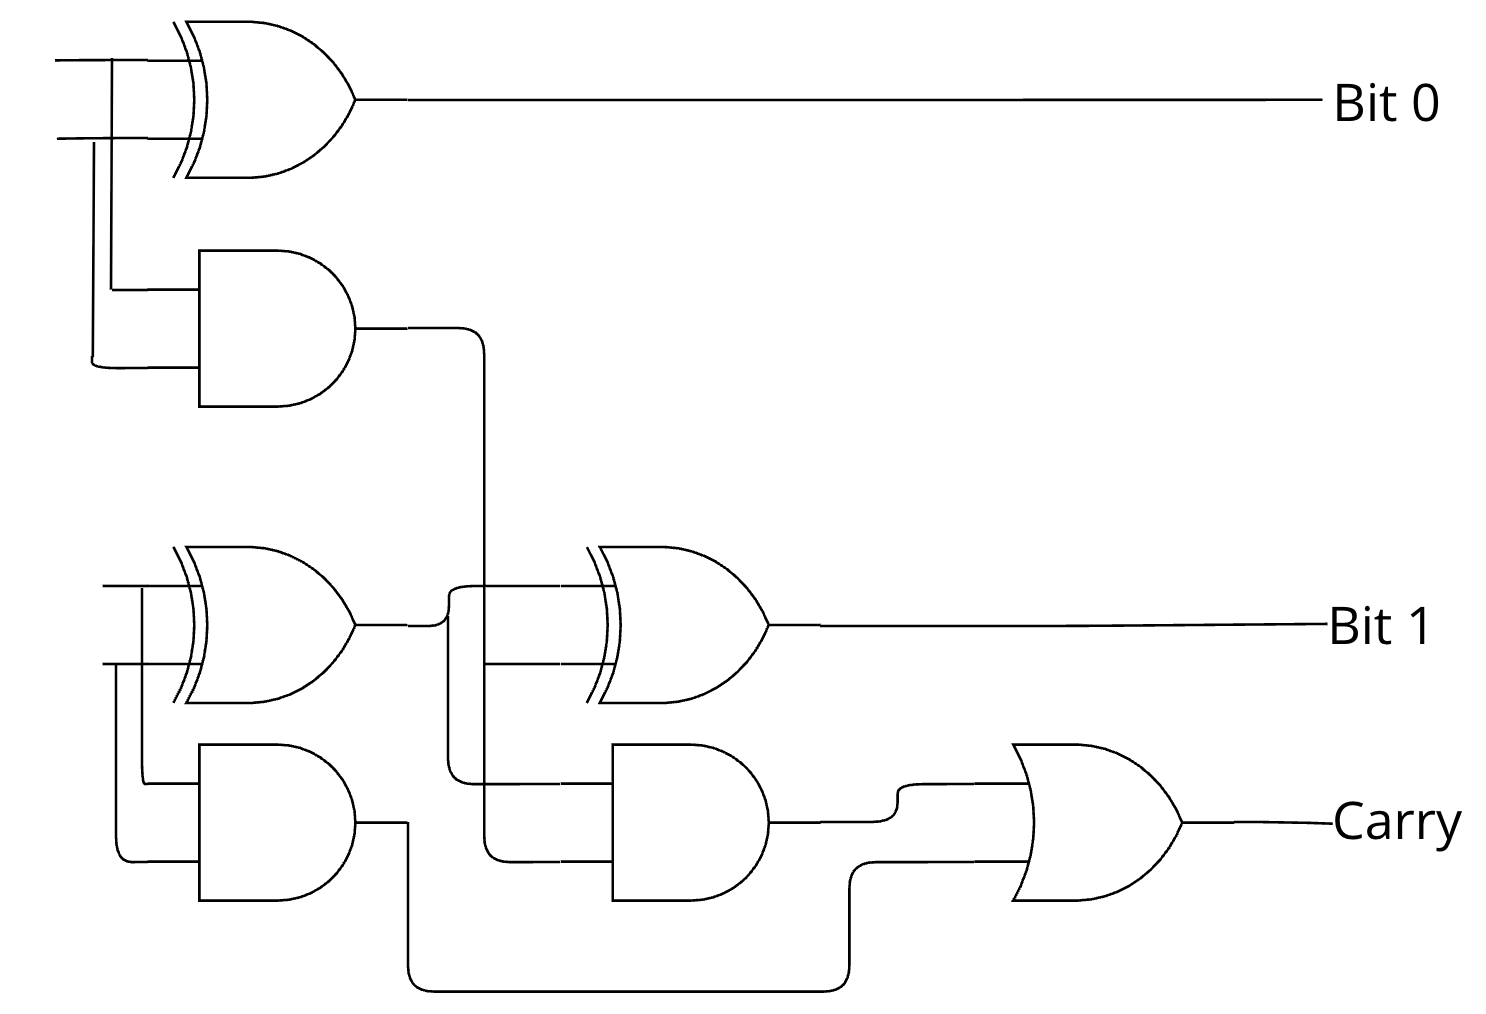
\includegraphics[scale=0.75]{2-bit-adder.png}
\end{center}
This circuit is not secure, but by replacing each gate by the GMW equivalent in Prelude, we can create an MPC protocol. Here we will more formally introduce the GMW protocol, as used as \textit{Prelude} language. 
{\footnotesize
\begin{verbatimtab}
exprfunctions:

RECON(x) { (m[x]@1 + m[x]@2) }

not(x){ x + 1 }

cmdfunctions:

xorgmw(z:string, x:string, y:string) {
   m[z]@1 := (m[x] + m[y])@1; 
   m[z]@2 := (m[x] + m[y])@2
} 
postcondition: (RECON(z) == RECON(x) + RECON(y))

notgmw(z:string, x:string) {
   m[z]@1 := m[x]@1;
   m[z]@2 := not(m[x])@2
}
postcondition: ( RECON(z) == not(RECON(x)) )
\end{verbatimtab}

}
Figure X \todo{REPLACE} defines the XOR and NOT as GMW-style \textit{Prelude} functions. For simplicity, the definition of the andgmw(x,y,z) function which uses oblivious transfer has beem omitted, but follows a similar structure. With these gate definitions, we built the Prelude implementation of the 2-bit Adder in Figure X \todo{REPLACE}. 
{\footnotesize
\begin{verbatimtab}
main() {
   xorgmw("z1", "x1", "y1"); // Bit 0 (least significant)
   andgmw("g1", "x1", "y1");
   xorgmw("g2", "x2", "y2");
   xorgmw("z2", "g2", "g1") // Bit 1 (most significant)
} 
postcondition: (|RECON("z2"), RECON("z1")| == BVAdd(|RECON("x2"), RECON("x1")|, |RECON("y2"), RECON("y1")|))
\end{verbatimtab}}
Note that the postcondition explicitly states the correctness property, that the output bit vector is equivalent to the sum of the two input bit vectors. The "$\vert$" syntax represents concatenation of bits into a larger bit vector and RECON() reconstructs the values by summing the shares of each secret. Given the body of main and the postcondition, the \textit{Prelude} tool passes the constraints to the SMT solver to automatically verify the protocol. \todo{Should there be more discussion of Prelude?}

\section{Methods}
In collaboration with PhD Student Steven Baldasty and Dr. Christian Skalka, we discussed and implemented changes to the \textit{Prelude} backend to include syntax for BVAdd(), BVSub(), and "$\vert$", the equivalent of BVConcat in the cvc5 solver. \todo{Should introduce cvc5 in smt section} This new functionality allows the tool to be used to verify circuits with bit vector representations of numbers as inputs for addition and subtraction. We made modifications to the Perl parsing script to include NOT gates as well as automatic generation of postconditions \todo{CITE PARSER IN REPO}. The parser was ran on Bristol Circuit text files for the 64-bit Adder and 64-bit Subtract \todo{CITE BRISTOL} circuits. With the GMW-style \textit{Prelude} function calls and BVAdd()/BVSub() postconditions, we implemented \textit{Prelude} code \todo{CITE repo circuit implementations} to automatically verify the correctness of the circuits containing hundreds of gates. \todo{Mention BVMult/64-bit multiplier as well?}
% \begin{itemize}
% \item cite GMW example from Prof. Skalka's paper
% \item cite Hoare logic definitions
% \item \cite{prelude-github}
% \end{itemize}

\section{Experiments and Results}
The \textit{Prelude} implementations of the 2-bit Adder, 64-bit Adder, and 64-bit Subtract Bristol Circuits were run on a personal MacBook Air with the M2 chip.
\begin{center}
\begin{tabular}{ |c|c|c|c|}
    \hline
    & 2-Bit Adder & 64-Bit Adder & 64-Bit Subtract\\
    \hline\hline
    Verification time (ms): & 28 & 3700 & 5300 \\
    \hline
\end{tabular}
\end{center}
\todo{Formatting of table, and figure out best practice for time (should I average it over x attempts?)}

\section{Conclusions and Future Work(?)}
Possibly talk about BVMult here or talk with Steven about what was holding it up on the VACC

\bibliographystyle{ACM-Reference-Format} % Best reference format?
\bibliography{draft}

\end{document}
